\documentclass{article}
\usepackage[top=1in, bottom=1in, left=1in, right=1in]{geometry}
\usepackage{url}
\usepackage{fancyhdr}
\pagestyle{fancy}
\usepackage{setspace}
\usepackage{graphicx}
\usepackage{verbatim}
\usepackage{listings}
\usepackage{xspace}
\usepackage[usenames,dvipsnames]{color}
\usepackage{tabularx}
\usepackage{multirow}

\newcommand{\us}{Joe Redmon and Doug Woos}
\newcommand{\class}{CSE 561 Project 1}

\newcommand{\todo}[1]{{{\color{blue}#1}}}

\title{\class} \author{\us}

\lhead{\class}
\rhead{\us}

%\newenvironment{outline}{}{}
\newenvironment{outline}{\comment}{\endcomment}

% macros
\begin{document}
\maketitle

\section{Implementation}
For modulation, We used an audio frequency shift keying (AFSK) scheme
modeled on that used by the Bell 202 modem. We used a two-tone scheme,
designating 1200Hz as the ``mark'' (indicating a 1) and 2400Hz as the
``space'' (indicating a 0). To decode the incoming audio data, we used
a simple zero-crossing algorithm, counting the number of times that
the waveform changes sign in order to determine its frequency over a
selected interval. We used a known preamble in order to determine the
offset at which to begin decoding.

We found that the transmission volume was critical in acheiving
acceptable error rates. We initially tried to transmit at the phone's
maximum volume, but found that it introduced far too much noise. We
reduced the volume until we could reliably find the preamble when the
phones were adjacent.

We experimented with a variety of symbols per bit, focusing on those
which yielded zero-crossing counts which were close to whole numbers
for the mark and space tones.

\section{Experiments}
We first tried to maximize our bitrate by reducing the symbols per
bit. When we held the phones directly adjacent to each other, we could
transmit with 37 symbols per bit, yielding a bitrate of 1225 bps with
an error rate of 1.5~\% when the phones were adjacent. However, we
could not transmit over any significant distance at this bitrate (we
got a bit error rate of just over 2~\% t 10cm). For the subsequent
experiments, we transmitted 74 symbols per bit for a bitrate of 596
bps.

For the distance experiments, we transmitted 1KB of randomly generated
data (using a consistent seed for repeatability and error detection)
from one phone to the other while varying the distance. We repeated
each experiment 10 times, and we report both the average and the
standard deviation. Our results are in
Figure~\ref{fig:distance_results}. Note that in several runs at larger
distances, the receiving phone failed to detect the preamble; we
counted this as 100~\% error rate (this accounts for the extremely
high variance at 40 and 60 cm).

At 30cm and 50cm, the bit error rate is under 2~\% (0.3~\% and 1.9~\%,
respectively). However, at 40cm a preamble-detection failure occurs.

\begin{figure}[h!]
  \label{fig:distance_results}
  \centering
  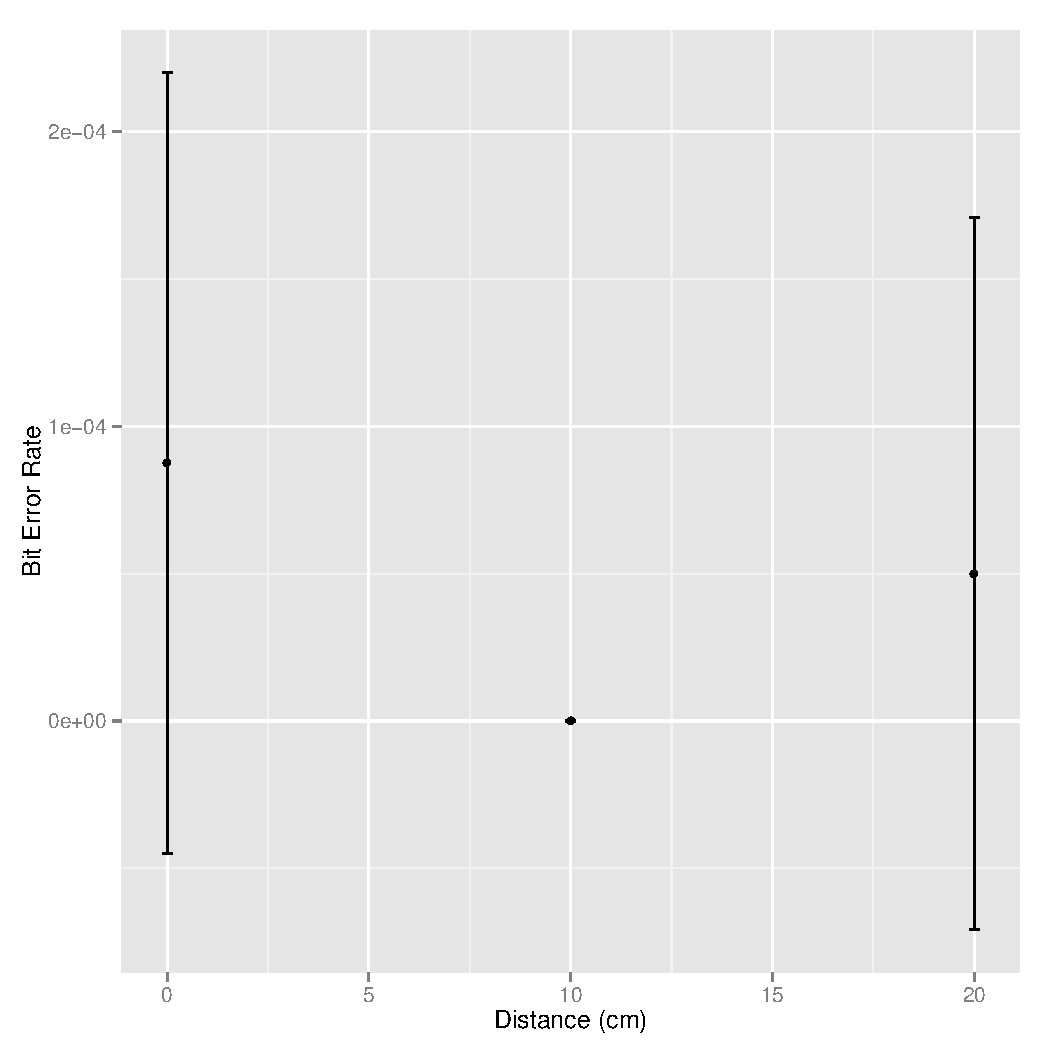
\includegraphics[width=0.8\textwidth]{figure.pdf}
  \caption{Bit error rate by distance. The points on the graph
    indicate mean error rate over 10 runs, while the bars indicate the
  standard deviation.}

\end{figure}
\end{document}
